\section{Task Design}

In this section the design and idea behind the task which was used in the experiment will be explained. It is intended to focus on the task design only without considering the virtual reality aspects and and actual procedure which will be described in the methods sections. But is has to be kept in mind that the task is intended to be implemented in a 3D virtual environment which allows participants to almost freely interact and move. The challenge of designing a problem for a spatial problem solving experiment in a virtual 3D space is to find a balance between limiting the options and degrees of freedom participants have, but also allowing them enough possibilities to apply individual strategies within those limitations.

When designing a task (or problem) for a problem solving experiment it is important to think about the complexity of the task. The literature differentiates between simple and complex problems. \cite{muesseler2015allgemeine}  A simple problem is characterized by having a clear initial  and goal state and all transitions and solution paths are known. Such problems suit very well to investigate heuristics, search processes and systematic errors in problem solving. The main advantage is that simple problems can be investigated well in experiments because they can be easily controlled. A complex problem is mainly characterized by the fact that it is more closely related to real life problems, which makes them harder to simulate in an experiment. It is important to understand that a simple problem must not necessearily be easy to solve. The adjective "simple" refers only to the fact that the problem's rules and its scope are limited to a few actions. The nine dot problem described before (Section \ref{sec:introduction} and Figure \ref{fig:ninedots}) can be categorized as a simple problem, because it is only possible to draw straight lines and it is not allowed to take the pen off the paper. Finding the solution still seems to be very difficult since only 10\% of the participants are able to solve the problem. \cite{muesseler2015allgemeine} 
Since we want to be able to quantify and compare performances of individuals and groups of two, the main requirement for the task  was that it is designed to have the characteristics of a simple problem. However, problem solving tasks in the 3D space are naturally pretty complex, because they allow all kinds of different movements and interactions. In the following the task components and rules will be described. Furthermore the theories behind this task will be explained to show why it suits to investigate and compare spatial problem solving for both individuals and groups of two.

\newpage

\subsection{Task components and goal} \label{sec:task_components}
In this section the task components, the initial state and the goal state will be described.
The components of the task are 10 cubes and a solution space with 4 slots to hold one cube each. Every cube has a color on each of its 6 faces. The same color can be assigned at most to two faces of a cube. Since the colors vary in each trial, a digit coding will be introduced in the following to describe the exact color configurations of all cubes. A color configuration of a cube consists of a mapping of all its faces to a digit code. Every digit code is a placeholder for a certain color. An example coding for one cube could look like this: 

\begin{center}
\textbf{front=1, back=0, left=2, right=0, top=7, bottom=8}
\end{center}


The cube faces can have 9 different colors and therefore a digit coding has been defined that ranges from 0 to 8. The 9 different colors are required because the distractor cubes need to be colored with some distractor colors, which are not part of the goal state. Since the resulting cuboid has 6 faces there are 6 colors which are actually part of the goal state. The other 3 colors are the distractor colors. The complete digit coding for all 9 cubes can be found in Table \ref{tab:digit_coding}.

\begin{table}
\begin{center}
    \begin{tabular}{| l | | l | l | l | l | l | l |  l |}
    \hline
    \textbf{Cube} & \textbf{front} & \textbf{back} & \textbf{left} & \textbf{right} & \textbf{top} & \textbf{bottom} & \textbf{type} \\ \hline
    A & 1 & 0 & 2 & 0 & 7 & 8 & starting/solution \\ \hline
    B & 0 & 3 & 2 & 0 & 7 & 8 & solution \\ \hline
    C & 0 & 3 & 0 & 4 & 7 & 8 & solution \\ \hline
    D & 1 & 0 & 0 & 4 & 7 & 8 & solution \\ \hline
    E & 2 & 0 & 0 & 3 & 7 & 8 & distractor \\ \hline
    F & 0 & 3 & 0 & 5 & 7 & 8 & distractor \\ \hline
    G & 0 & 4 & 0 & 5 & 7 & 8 & distractor \\ \hline
    H & 0 & 3 & 0 & 6 & 7 & 8 & distractor \\ \hline
    I & 0 & 5 & 1 & 0 & 7 & 8 & distractor \\ \hline
    \end{tabular}
\end{center}
\caption{Digit coding of the color configuration for all cubes.}
\label{tab:digit_coding}
\end{table}

After taking a closer look at Table \ref{tab:digit_coding} one can see that the digits 0, 7 and 8 are represented in each cube. This is one of the simplifications which was made in order to make sure the task is not too complex and has the characteristics of a simple problem. The digit 0 is always mapped to gray because gray is defined to be the color of the faces that must point to the inside of the solution space. The digit 7 is always mapped to white because it defines the top of each cube in the solution space. And the digit 8 is always mapped to black because it defines the bottom of each cube in the solution space. Therefore the top and bottom of the solution space are the same in each trial (white and black). Only the colors of the side faces are variable between trials and therefore allow to generate different instances of the same task that only differ in color of the cube's side faces. For the complete overview of predefined and variable colors refer to Table \ref{tab:color_mapping}.

\begin{table}
\begin{center}
    \begin{tabular}{| l | l |}
    \hline
    \textbf{Digit code} & \textbf{color} \\ \hline
    0 & gray \\ \hline
    1 & variable \\ \hline
    2 & variable \\ \hline
    3 & variable \\ \hline
    4 & variable \\ \hline
    5 & variable \\ \hline
    6 & variable \\ \hline
    7 & white \\ \hline
    8 & black \\ \hline
    \end{tabular}
\end{center}
\caption{Predefined and variable colors for digit codes.}
\label{tab:color_mapping}
\end{table}

The solution space consists of 4 slots which have the same size as a cube. The slots are arranged in a square from a top down view. In the initial state of the task the starting cube is already placed into the correct position and orientation of the solution space and the remaining 8 cubes are placed around the solution space. Furthermore, the remaining 8 cubes are rotated and positioned differently in each trial so that participants can not learn at which position the cubes for the solution are located. (see Figure \ref{fig:vr_task_initialstate})

\begin{figure}[h]
\centering
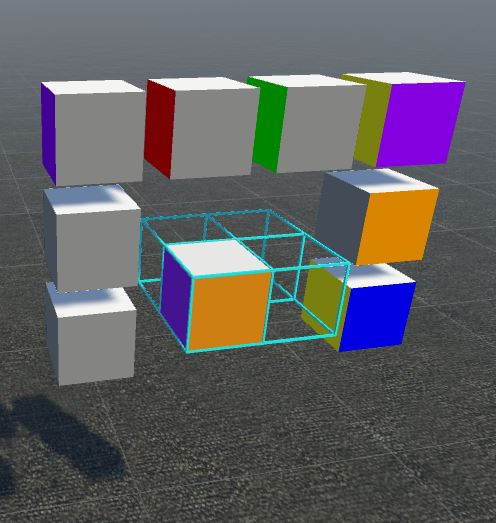
\includegraphics[width=0.5\textwidth]{vr_task_initialstate}
\caption{Initial state of the task: In the center - the solution space in light blue with the starting cube. Surrounding the solution space - the 9 remaining cubes to interact with. }
\label{fig:vr_task_initialstate}
\end{figure}

\newpage

The goal state of the task is achieved when all slots of the solution space are filled with a cube and all 6 faces of the resulting cuboid are colored differently but also unicolored each. The colors of the goal state displayed in Figure \ref{fig:vr_task_goalstate} are the following (not all colors can be seen because of the perspective):

\begin{center}
\textbf{front=orange, back=red, left=purple, right=blue, top=white, bottom=black}
\end{center}

\begin{figure}[h]
\centering
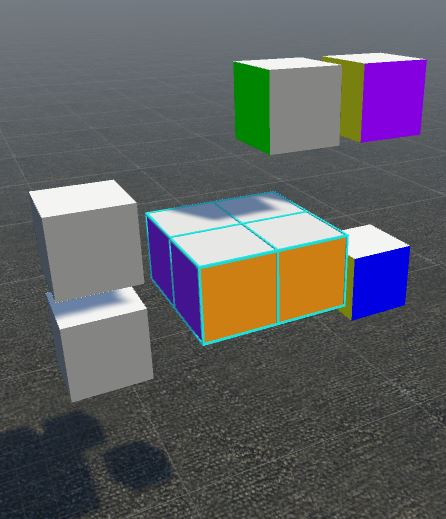
\includegraphics[width=0.5\textwidth]{vr_task_goalstate2_4}
\caption{Goal state of the task: All slots of the solution space are filled with a cube and all 6 faces of the resulting cuboid are differently colored, but also unicolored each. }
\label{fig:vr_task_goalstate}
\end{figure}

There are only 3 cubes that fit to achieve the goal state. Each of those 3 cubes fits exactly into one specific slot of the solution space. Those 3 cubes will be referred to as the "goal cubes". The remaining 6 cubes will be referred to as the "distractor cubes".

\subsection{Task rules} \label{sec:task_rules}
The most important rule of the task is that the cubes have to be put into the slots of the solution space in a certain sequence.
This sequence is shown in Figure \ref{fig:task_rules}). When participants see the task in front of them, the starting cube is always located in the left slot close to the participant (1). The second slot in the sequence - which is actually the first slot participants fill themselves - is the the slot behind the first slot (2). The third slot is the to the right of the starting cube (3). And the fourth slot is behind the third slot (4). When participants need to remove cubes, they have to do it in the reverse order. One example situation in which they need to remove cubes will be described in the following: when the second and third slot of the solution space have already been filled, but there exists no 4th cube to make the solution complete, participants first need to remove the cube from the 3rd slot. Optionally they can try to replace it with another cube to see if it leads to the solution. If they decide to keep the third cube removed, they can also remove the second cube. It is not allowed to remove the second cube as long as there still is a cube placed into the third slot. 

\begin{figure}[h]
\centering
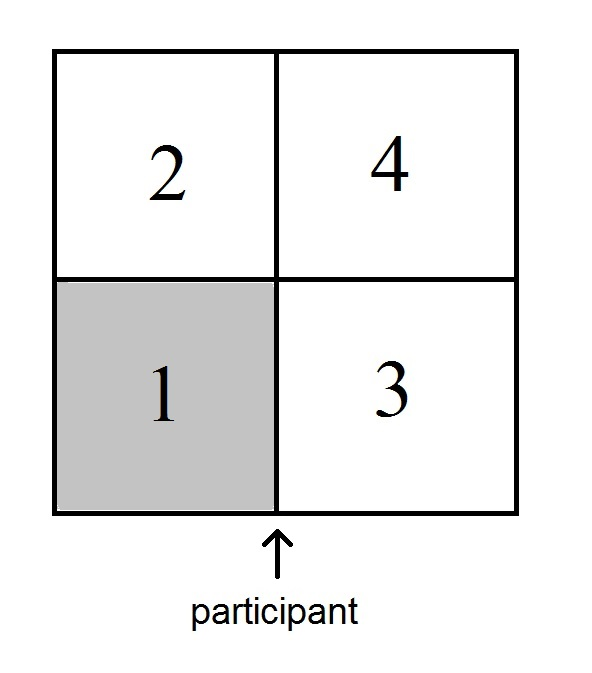
\includegraphics[width=0.5\textwidth]{task_rules}
\caption{Top down view of the task, showing the sequence in which cubes have to be but into the slots of the solution space from 1 to 4. }
\label{fig:task_rules}
\end{figure}

\subsection{Task theory}
An important aspect of the task design was to reduce the variations of how participants could solve the task. In this section the theories and main concepts of the task design will be explained in order to show that it suits well to perform controlled spatial problem solving experiments.

\subsubsection{Binary tree structure}
The main characteristic of the task is that there are several partial solutions to the problem because of the distractor cubes. Those partial solutions and the actual solution can be displayed in a binary tree. (see Figure \ref{fig:vr_tree}) The binary tree is representing the 4 paths which a participant may use in order to find the solution. The root node of the tree represents the initial state of the task showing the colors of starting cube in the solution space. Since the task was designed to have a binary tree structure there are always two options to put in a cube in a slot, following the given sequence. Therefore following two nodes represent the two options to place a second cube. The same applies to the next level of the tree. The solution space has been rotated for each node in a way that the relevant colors are visible. The bottom nodes show the possible end state of each path. It can be seen that only the right path leads to the goal state.

\begin{figure}[h]
\centering
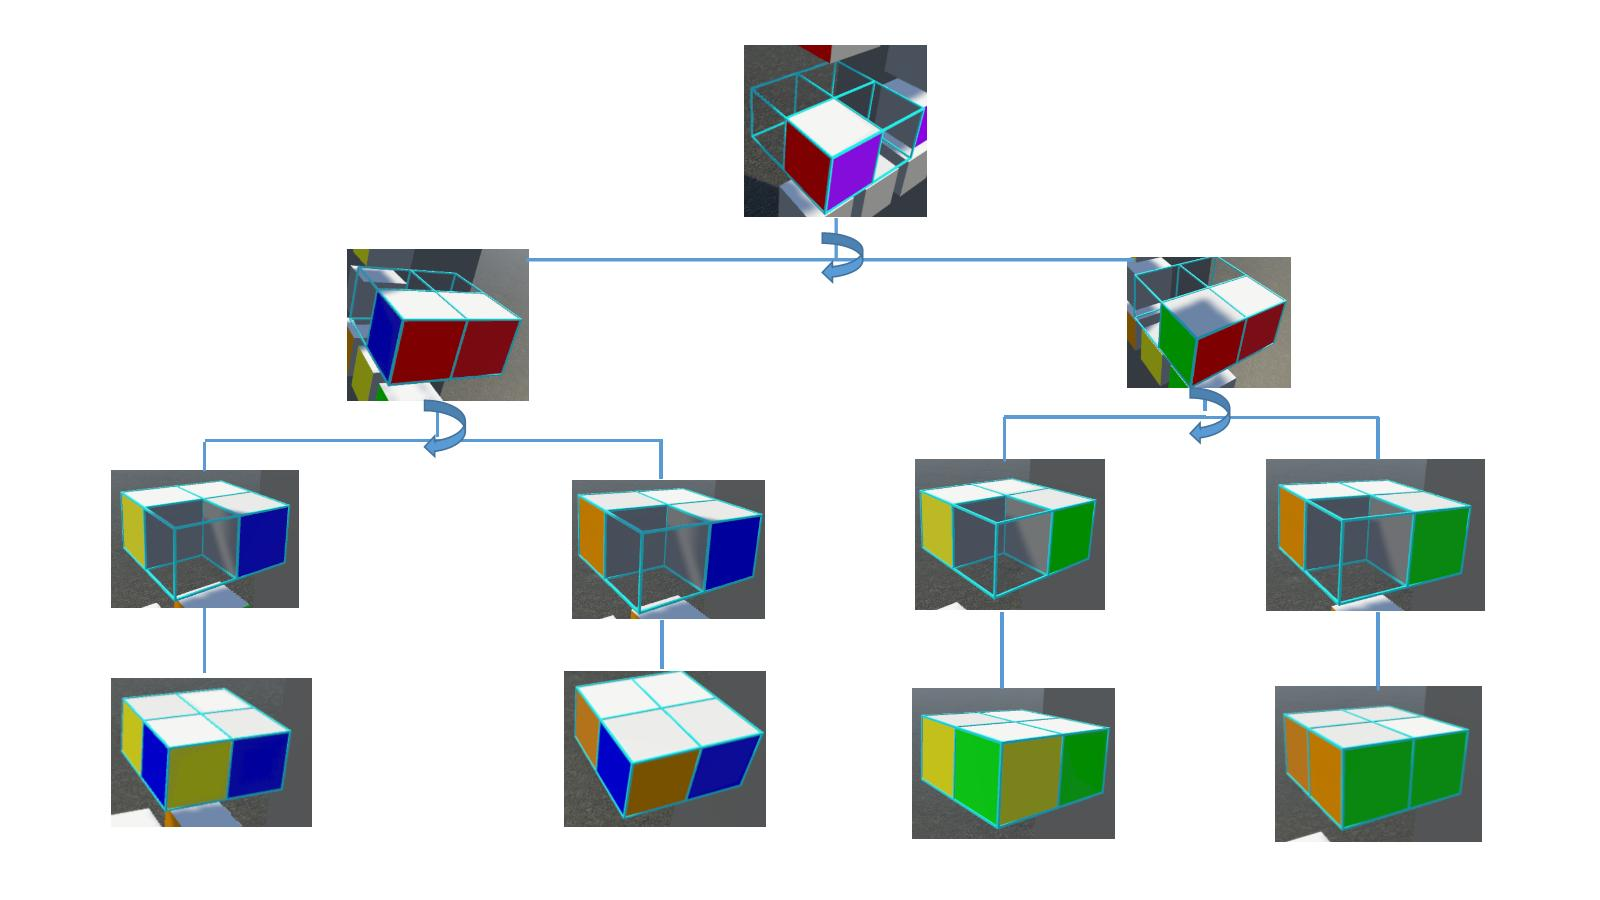
\includegraphics[width=1.0\textwidth]{vr_tree}
\caption{Binary tree structure of the different solution paths of the task.}
\label{fig:vr_tree}
\end{figure}

Since distractor cubes are colored in a way that they appear to be part of the solution, participants can not instantly find the solution (unless they are lucky). The idea of the task is that participants have to apply a try and error strategy, but in a very systematic way. In order direct the participants towards this systematic try and error strategy, they receive the instructions to follow the sequence in which cubes have to be put into (and removed from) the solution space (as described in Section \ref{sec:task_rules}). As it can be seen in Figure \ref{fig:vr_tree} there are 4 possible paths in the tree to fill the solution space. But only one path leads to the correct solution and therefore there is a 25\% chance to instantly solve the task - assuming participants always stick to the sequence rules. In the worst case they need to try all 4 paths to find the solution. This also means that by design each task trial should be possible to be solved within a certain amount of time, which is beneficial to compare the time performances between the individuals and groups of two. 

Besides the predictable solution time, the tree structure also allows to precisely quantify the actual error of participants. The amount of paths within the tree participants need to try is random and therefore not controlled. This means the actual performance is both flawless when participants need to try only 1 or all 4 paths of the tree. An actual error occurs only when participants repeatedly try the same path of the tree. Such an error can be ascribed to the working memory since in this case participants clearly forgot that they tried the same path before.

\subsubsection{Simplifications}
One simplification of the task was to have only one solution. This has been achieved by designing the task in a way that there are only the 3 goal cubes which are part of the solution. None of the goal cubes can be exchanged by another cube so that for each trial all participants have the exact same goal state.

Furthermore some of the cube colors always have the same meaning and therefore support the participants in finding the right orientation for each cube within the solution space. White always indicated the top face of a cube in the solution space, black always indicated the bottom face of a cube in the solution space. Thus, participants only need to find the correct orientation of a cube in the vertical rotation axis. The gray faces always indicate the faces which point into the center of the solution space and have a similar function because they help to correctly orient the cubes within the solution space.

\subsubsection{Trials}
Both in the single and group condition participants have to solve 20 trials of the task. The benefit of the task design is that 20 different instances of the task can be generated. And the instances only differ in colors as described in Section \ref{sec:task_components} Thus the complexity or difficulty is the same for each trial and at the same time participants can not learn the position or the colors of cubes in the initial state, since they change from trial to trial. For each participant we use a randomized order of the 20 trials, but the pool of trials is the same.

Another aspect of the repetitive execution of the same task is that participants are supposed to improve over time, because they are expected to understand the tree like structure of the task and therefore get better at avoiding errors (trying the same path more than once). This aspect of the task design is only mentioned for completeness, but will not be further discussed in this study.


\subsubsection{Summary}
Both the binary tree structure of the task and the simplifications reduce its complexity so that it is more controlled. This makes it is easier to analyze the performance of participants. The task design is intended to be suitable for different kinds of research questions in the field spacial problem solving. In this work the focus is the comparison between the performances of individuals and groups of two.